\documentclass[varwidth=true, border=2pt]{standalone}
\usepackage{tikz}
\usetikzlibrary{shapes, calc} 
\begin{document}
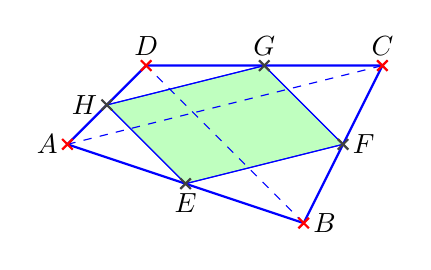
\begin{tikzpicture}
    % Define display style
    \tikzstyle{cross}=[cross out, draw, solid, red, inner sep=1.5pt, thick]
    \tikzstyle{diagonals}=[dashed, blue]

    % Define coordinates
    \newcommand\AX{0}
    \newcommand\AY{1}

    \newcommand\BX{3}
    \newcommand\BY{0}

    \newcommand\CX{4}
    \newcommand\CY{2}

    \newcommand\DX{1}
    \newcommand\DY{2}

    % Create shortcuts for coordinates and draw labels
    \coordinate[label=left:$A$]  (A) at (\AX, \AY);
    \coordinate[label=right:$B$] (B) at (\BX, \BY);
    \coordinate[label=above:$C$] (C) at (\CX, \CY);
    \coordinate[label=above:$D$] (D) at (\DX, \DY);

    \coordinate[label=below:$E$] (E) at ({(\AX+\BX)/2}, {(\AY+\BY)/2});
    \coordinate[label=right:$F$] (F) at ({(\BX+\CX)/2}, {(\BY+\CY)/2});
    \coordinate[label=above:$G$] (G) at ({(\CX+\DX)/2}, {(\CY+\DY)/2});
    \coordinate[label=left:$H$] (H) at ({(\DX+\AX)/2}, {(\DY+\AY)/2});

    % Draw the rectangle
    \draw[blue, thick]  (A) -- (B) -- (C) -- (D) -- (A);

    % Draw the background of the parallelogram
    \draw[blue, fill=green!25] (E) -- (F) -- (G) -- (H) -- (E);

    % Draw the diagonals
    \draw[diagonals] (A) -- (C);
    \draw[diagonals] (B) -- (D);

    % Draw the parallelogram itself
    \draw[blue] (E) -- (F) -- (G) -- (H) -- (E);

    % Draw the crosses for each edge
    \foreach \coordinateName in {A, B, C, D}
        \node[cross] at (\coordinateName) {};

    \foreach \coordinateName in {E, F, G, H}
        \node[cross, gray!50!black] at (\coordinateName) {};
  \end{tikzpicture}
\end{document}
